
% This LaTeX was auto-generated from MATLAB code.
% To make changes, update the MATLAB code and republish this document.

\documentclass{article}
\usepackage{graphicx}
\usepackage{color}

\usepackage[T1]{fontenc} % Can use danish characters       
\usepackage[hidelinks]{hyperref} % TOC is click-able
\usepackage[left=3cm,right=2cm,top=2.5cm,bottom=2cm]{geometry}
\usepackage{amsmath}
\DeclareMathOperator*{\argmin}{arg\,min}

\sloppy
\definecolor{lightgray}{gray}{0.5}
\setlength{\parindent}{0pt}

\begin{document}

\includegraphics[width=\linewidth]{Frontpage.pdf}
\tableofcontents
\newpage

\section{Exercise 1}

\begin{par}
Optimization using the simplex method:
\end{par} \vspace{1em}
\begin{verbatim}
% The augmented matrix:
clc; clear;
A = [1  2  0  1  0  0  0  28;
     2  0  4  0  1  0  0  16;
     0  1  1  0  0  1  0  12;
    -2 -5 -3  0  0  0  1  0]
\end{verbatim}

        \color{lightgray} \begin{verbatim}
A =

     1     2     0     1     0     0     0    28
     2     0     4     0     1     0     0    16
     0     1     1     0     0     1     0    12
    -2    -5    -3     0     0     0     1     0

\end{verbatim} \color{black}
    \begin{par}
We want to bring $x_2$ in, since $A(4,2) < A(4,3) < A(4,1)$, and thus increases $A(4,8)$ the most. The pivot row should be $A(3,2)$, since $$\frac{A(3,8)}{A(3,2)} = 12 < \frac{A(1,8)}{A(1,2)} = 14$$
\end{par} \vspace{1em}
\begin{verbatim}
A(1,:) = A(1,:)-2*A(3,:);
\end{verbatim}
\begin{verbatim}
A(4,:) = A(4,:) + 5*A(3,:)
\end{verbatim}

        \color{lightgray} \begin{verbatim}
A =

     1     0    -2     1     0    -2     0     4
     2     0     4     0     1     0     0    16
     0     1     1     0     0     1     0    12
    -2     0     2     0     0     5     1    60

\end{verbatim} \color{black}
    \begin{par}
Next, we bring in $x_1$, since $A(4,1)$ is the only negative value in $A(4,:)$. $A(1,1)$ is the new pivot, since $$\frac{A(1,8)}{A(1,1)} = 4 < \frac{A(2,8)}{A(2,1)} = 8$$
\end{par} \vspace{1em}
\begin{verbatim}
A(2,:) = A(2,:) -2*A(1,:);
\end{verbatim}
\begin{verbatim}
A(4,:) = A(4,:) + 2*A(1,:)
\end{verbatim}

        \color{lightgray} \begin{verbatim}
A =

     1     0    -2     1     0    -2     0     4
     0     0     8    -2     1     4     0     8
     0     1     1     0     0     1     0    12
     0     0    -2     2     0     1     1    68

\end{verbatim} \color{black}
    \begin{par}
Last, we bring in $x_3$, with pivot $A(2,3)$, since $A(1,3)$ is negative and $$\frac{A(2,8)}{A(2,1)} = 1 < \frac{A(3,8)}{A(3,1)} = 12$$
\end{par} \vspace{1em}
\begin{verbatim}
A(2,:) = A(2,:)/8;
\end{verbatim}
\begin{verbatim}
A(1,:) = A(1,:) + 2*A(2,:);
\end{verbatim}
\begin{verbatim}
A(3,:) = A(3,:) - A(2,:);
\end{verbatim}
\begin{verbatim}
A(4,:) = A(4,:) + 2*A(2,:)
\end{verbatim}

        \color{lightgray} \begin{verbatim}
A =

  Columns 1 through 7

    1.0000         0         0    0.5000    0.2500   -1.0000         0
         0         0    1.0000   -0.2500    0.1250    0.5000         0
         0    1.0000         0    0.2500   -0.1250    0.5000         0
         0         0         0    1.5000    0.2500    2.0000    1.0000

  Column 8

    6.0000
    1.0000
   11.0000
   70.0000

\end{verbatim} \color{black}
    \begin{par}
Thus the maximum of the problem is 70, which is achieved when $x_1 = 6$, $x_2 = 1$ and $x_3 = 11$.
\end{par} \vspace{1em}

\newpage
\section{Exercise 2}

\begin{par}
Minimizing the function $f(x) = x_1^2+3*x_2^2-2*x_1*x_2+3*x_2$. 1. Write f on the form: $\frac{1}{2}*x^T*Q*x-x^T*b$:
\end{par} \vspace{1em}
\begin{verbatim}
Q = [2 -2;-2 6]
b = [0;-3]
\end{verbatim}

        \color{lightgray} \begin{verbatim}
Q =

     2    -2
    -2     6


b =

     0
    -3

\end{verbatim} \color{black}
    \begin{par}
2. Sketch the levels set for f and the gradient of f in the point $(1,1)^T$ in a $x_1,x_2$-coordinate system.
\end{par} \vspace{1em}
\begin{verbatim}
[x1, x2] = meshgrid(-10:1:10,-10:1:10);
x = [x1;x2];
f1 = x1.^2+3*x2.^2-2*x1.*x2+3*x2;
[C,h1] = contour(x1,x2,f1,[0 3 10 50 100 200 400]);
set(h1,'ShowText','on','TextStep',get(h1,'LevelStep')*2)
colormap cool
title('Level sets of f (x)')
xlabel('x1')
ylabel('x2')
\end{verbatim}

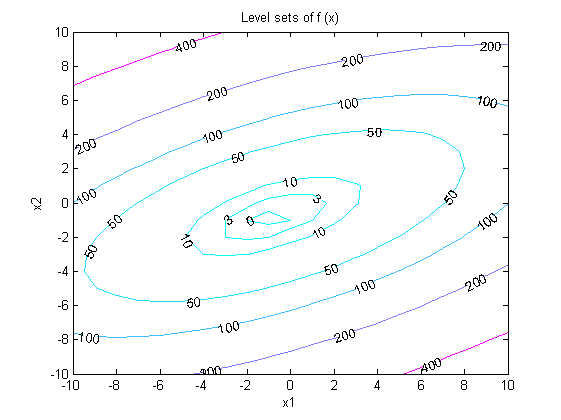
\includegraphics [width=4in]{Assignment10783_01.png}
\begin{par}
Gradient of f in the point $(1,1)^T$:
\end{par} \vspace{1em}
\begin{verbatim}
g1 = Q*[1;1]-b
\end{verbatim}

        \color{lightgray} \begin{verbatim}
g1 =

     0
     7

\end{verbatim} \color{black}
    \begin{par}
3. Find all point satisfying the FONC. Do these points satisfy the SONC?
\end{par} \vspace{1em}
\begin{par}
The gradient of f is found to be: $$f'(x)= Q*x-b$$
\end{par} \vspace{1em}
\begin{par}
Finding the point satisfying the FONC equals solving the following: $$Q*x-b = 0$$
\end{par} \vspace{1em}
\begin{par}
This gives the following point:
\end{par} \vspace{1em}
\begin{verbatim}
x = inv(Q)*b
\end{verbatim}

        \color{lightgray} \begin{verbatim}
x =

   -0.7500
   -0.7500

\end{verbatim} \color{black}
    \begin{par}
The Hessian is found to be $F(x) = Q$. Thus, the SONC is to test whether Q \ensuremath{>} 0:
\end{par} \vspace{1em}
\begin{verbatim}
format short
eigs(Q)
\end{verbatim}

        \color{lightgray} \begin{verbatim}
ans =

    6.8284
    1.1716

\end{verbatim} \color{black}
    \begin{par}
Since all eigenvalues of Q is positive, Q \ensuremath{>} 0 then the SONC is satisfied in all points satisfiying the FONC.
\end{par} \vspace{1em}
\begin{par}
4. Find the minimum of f over $R^2$
\end{par} \vspace{1em}
\begin{par}
Since both the FONC and SOSC is satisfied by the previous piont, this is the global minimum:
\end{par} \vspace{1em}
\begin{verbatim}
x
\end{verbatim}

        \color{lightgray} \begin{verbatim}
x =

   -0.7500
   -0.7500

\end{verbatim} \color{black}
    
\newpage
\section{Exercise 3}

\begin{par}
Newtons method
\end{par} \vspace{1em}
\begin{par}
Given the function $f(x) = \frac{1}{2}*x^2-cos(x)$.
\end{par} \vspace{1em}
\begin{par}
1. Sketch the graph of $f$ and find the 1. and 2. derivative of $f$:
\end{par} \vspace{1em}
\begin{verbatim}
syms x;
f2(x) = 0.5*x.^2-cos(x);
ezplot(f2)
title('f(x)');
ylabel('f(x)');
xlabel('x');
\end{verbatim}

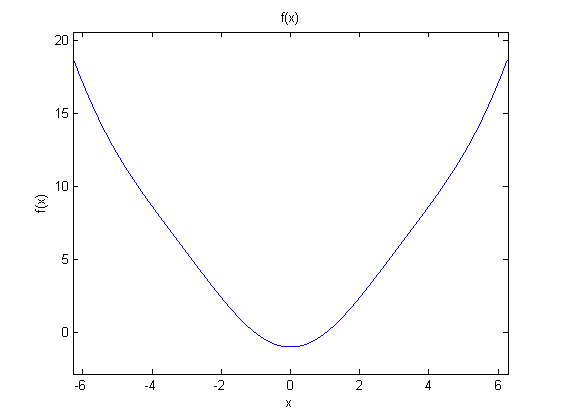
\includegraphics [width=4in]{Assignment10783_02.png}
\begin{par}
First derivative:
\end{par} \vspace{1em}
\begin{verbatim}
g2(x) = diff(f2)
\end{verbatim}

        \color{lightgray} \begin{verbatim} 
g2(x) =
 
x + sin(x)
 
\end{verbatim} \color{black}
    \begin{par}
Second derivative:
\end{par} \vspace{1em}
\begin{verbatim}
F2(x) = diff(g2)
\end{verbatim}

        \color{lightgray} \begin{verbatim} 
F2(x) =
 
cos(x) + 1
 
\end{verbatim} \color{black}
    \begin{par}
2. Use Newtons method to find the minimizer of $f$, where:
\end{par} \vspace{1em}
\begin{verbatim}
x0 = 0.25;
\end{verbatim}
\begin{par}
Newtons method uses the formular $$x^{(k+1)} = x^k-\frac{f'(x^k)}{f''(x^k)}$$ when both the first and second derivatives are known.
\end{par} \vspace{1em}
\begin{verbatim}
x1 = eval(x0 - g2(x0)/F2(x0))
x2 = eval(x1 - g2(x1)/F2(x1))
x3 = eval(x2 - g2(x2)/F2(x2))
\end{verbatim}

        \color{lightgray} \begin{verbatim}
x1 =

   -0.0026


x2 =

   3.0277e-09


x3 =

     0

\end{verbatim} \color{black}
    \begin{par}
Note that the accuracy
\end{par} \vspace{1em}
\begin{verbatim}
er = abs(x3-x2)
\end{verbatim}

        \color{lightgray} \begin{verbatim}
er =

   3.0277e-09

\end{verbatim} \color{black}
    \begin{par}
satisfy the needed accuracy of $e < 10^{(-5)}$. Thus, the needed number of iterations is \textit{3}.
\end{par} \vspace{1em}

\newpage
\section{Exercise 4}

\begin{par}
Steepest descent algorithm: Given the quadratic function from exercise 2:
\end{par} \vspace{1em}
\begin{verbatim}
syms xx1 xx2;
x = [xx1;xx2];
Q = [2 -2;-2 6];
b = [0;-3];
f3(x) = 0.5*x.'*Q*x-x.'*b;
\end{verbatim}
\begin{par}
The initail starting point is:
\end{par} \vspace{1em}
\begin{verbatim}
x0 = [1;1];
\end{verbatim}
\begin{par}
The gradient of $f$ is:
\end{par} \vspace{1em}
\begin{verbatim}
g3(x) = Q*x-b;
\end{verbatim}
\begin{par}
To compute $x^1$ we need $$\alpha_0 = \argmin_{\alpha \geq 0} f(x^0-\alpha \bigtriangledown f(x^0)) = \Phi(\alpha)$$
\end{par} \vspace{1em}
\begin{verbatim}
syms a;
arg = x0-a*g3(x0(1),x0(2));
Phi0(a) = f3(arg(1),arg(2));
\end{verbatim}
\begin{par}
To find $\alpha_0$ we use the FONC and plot the graph of $\Phi(\alpha)$, to ensure it is a minimium
\end{par} \vspace{1em}
\begin{verbatim}
a0 = solve(diff(Phi0(a)) == 0)
ezplot(Phi0(a))
title('Phi2(a)');
\end{verbatim}

        \color{lightgray} \begin{verbatim} 
a0 =
 
1/6
 
\end{verbatim} \color{black}
    
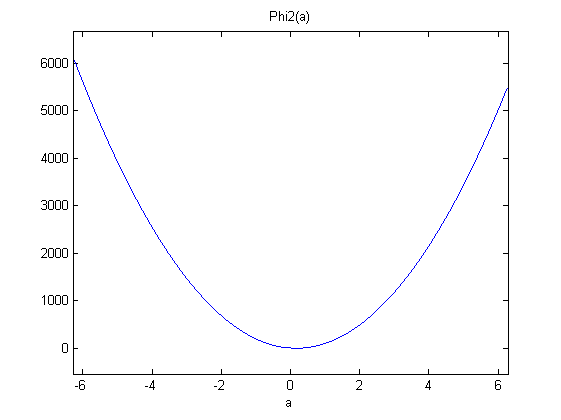
\includegraphics [width=4in]{Assignment10783_03.png}
\begin{par}
Now we find $x^1$:
\end{par} \vspace{1em}
\begin{verbatim}
x1 = x0-a0*g3(x0(1),x0(2))
\end{verbatim}

        \color{lightgray} \begin{verbatim} 
x1 =
 
    1
 -1/6
 
\end{verbatim} \color{black}
    \begin{par}
Now we use same approach to find $x^2$ and $x^3$:
\end{par} \vspace{1em}
\begin{verbatim}
arg = x1-a*g3(x1(1),x1(2));
Phi1(a) = f3(arg(1),arg(2));
a1 = solve(diff(Phi1(a)) == 0)
ezplot(Phi1(a))
title('Phi1(a)');
x2 = x1-a1*g3(x1(1),x1(2))
\end{verbatim}

        \color{lightgray} \begin{verbatim} 
a1 =
 
1/2
 
 
x2 =
 
 -1/6
 -1/6
 
\end{verbatim} \color{black}
    
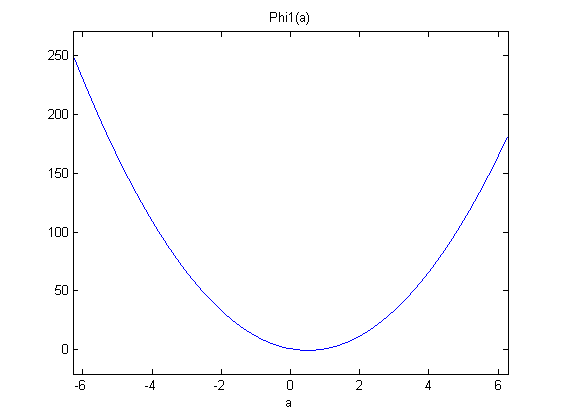
\includegraphics [width=4in]{Assignment10783_04.png}
\begin{verbatim}
arg = x2-a*g3(x2(1),x2(2));
Phi2(a) = f3(arg(1),arg(2));
a2 = solve(diff(Phi2(a)) == 0)
ezplot(Phi2(a))
title('Phi2(a)');
x3 = x2-a2*g3(x2(1),x2(2))
\end{verbatim}

        \color{lightgray} \begin{verbatim} 
a2 =
 
1/6
 
 
x3 =
 
 -1/6
 -5/9
 
\end{verbatim} \color{black}
    
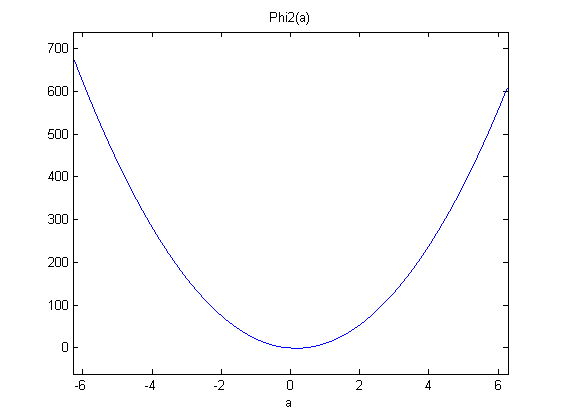
\includegraphics [width=4in]{Assignment10783_05.png}
\begin{par}
2. Does the steepest descent algorithm converge?
\end{par} \vspace{1em}
\begin{par}
From Theorem 8.2 in the Chong book, the steepest descent algorithm will always converge. This is also clearly evident, when looking at the graph of $f(x)$:
\end{par} \vspace{1em}
\begin{verbatim}
ezsurf(f3(xx1,xx2))
\end{verbatim}

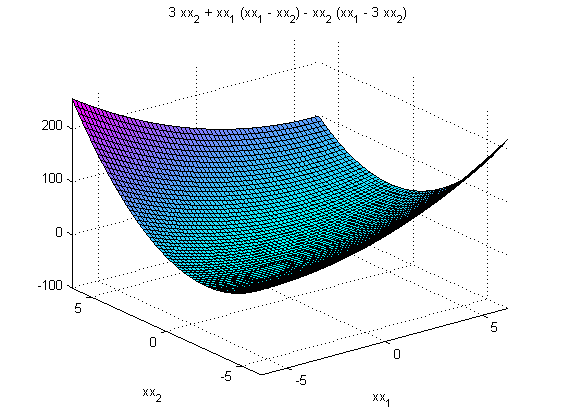
\includegraphics [width=4in]{Assignment10783_06.png}
\newpage
\begin{par}
3. Use a fixed-step size algorithm, what step size should be used to ensure convergence?
\end{par} \vspace{1em}
\begin{par}
Since Q is symmetric, we know that $f(x)$ converges if the following inequality is satisfied: $$0 < \alpha < \frac{2}{\lambda_{max}(Q)}$$
\end{par} \vspace{1em}
\begin{verbatim}
lambda_max  = max(eigs(Q))
\end{verbatim}

        \color{lightgray} \begin{verbatim}
lambda_max =

    6.8284

\end{verbatim} \color{black}
    \begin{par}
Thus, as long as $0 < \alpha < 6.8284$ the algorithm will converge.
\end{par} \vspace{1em}

\newpage
\section{Exercise 5}

\begin{par}
Data-fitting problem
\end{par} \vspace{1em}
\begin{par}
1. Calculate and write out $J(x)$
\end{par} \vspace{1em}
\begin{par}
Since the number of samples is unknown, we calculate $J(x)$ column-wise, as a function of $t_i$:
\end{par} \vspace{1em}
\begin{verbatim}
syms yi A ti s;
x = [A,s];
Jc1(x) = diff(yi-A*exp(-(ti^2)/(s^2)),A)
Jc2(x) = diff(yi-A*exp(-(ti^2)/(s^2)),s)
\end{verbatim}

        \color{lightgray} \begin{verbatim} 
Jc1(A, s) =
 
-exp(-ti^2/s^2)
 
 
Jc2(A, s) =
 
-(2*A*ti^2*exp(-ti^2/s^2))/s^3
 
\end{verbatim} \color{black}
    \begin{par}
2. Fill in the missing code, and plot decision variables $A$ and $\sigma$ as a function of iteration number.
\end{par} \vspace{1em}
\begin{par}
Simulation dataset
\end{par} \vspace{1em}
\begin{verbatim}
t=(-2:.01:2);
x_gold=[1;.1];
y=x_gold(1)*exp(-(t).^2/x_gold(2)^2);
y=y+.03*randn(size(y));
figure(1)
plot(y,'.b'); hold on;
xlabel('ti');
ylabel('yi');
xx=[];
x=x_gold+[.9;.9];

for k=1:75
 J= [               -exp(-(t).^2/x(2)^2);
       -(2*x(1)*t.^2.*exp(-(t).^2/x(2)^2))/x(2)^3].';

    f = x(1)*exp(-(t).^2/x(2)^2);
    r=y-f;

    x=x-(J.'*J)^(-1)*(J.'*r.');
    xx=[xx,x];
    plot(f)
    pause(.1)
end
figure(2)
plot(xx(1,:),'.r');hold on;
plot(xx(2,:),'.g');
xlabel('Number of iterations');
ylabel('A and sigma values');
\end{verbatim}

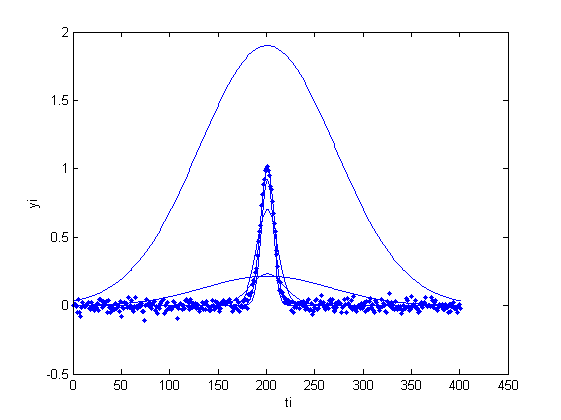
\includegraphics [width=4in]{Assignment10783_07.png}

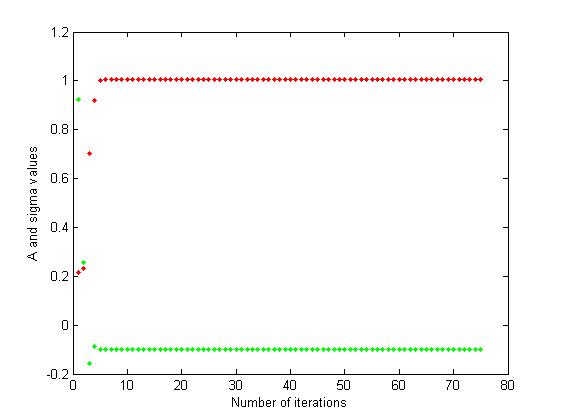
\includegraphics [width=4in]{Assignment10783_08.png}
\begin{par}
Note that $\sigma$ is found to be $-0.1$, whereas the function is defined with $\sigma = .1$ This is the case, since $\sigma = \pm 0.1$ both solves the datafitting problem, since $\sigma$ is squared everywhere it is used.
\end{par} \vspace{1em}

\newpage
\section{Exercise 6}

\begin{par}
Conjugate gradient algorithm
\end{par} \vspace{1em}
\begin{par}
Given the function $f$:
\end{par} \vspace{1em}
\begin{verbatim}
syms xx1 xx2;
x = [xx1;xx2];
Q = [2 -2;-2 6];
b = [0;-3];
f4(x) = 0.5*x.'*Q*x-x.'*b;
\end{verbatim}
\begin{par}
The initail starting point is:
\end{par} \vspace{1em}
\begin{verbatim}
x0 = [1;1];
\end{verbatim}
\begin{par}
Calculate the first 3 steps in the conjugate gradient method.
\end{par} \vspace{1em}
\begin{par}
The gradient of $f$ is:
\end{par} \vspace{1em}
\begin{verbatim}
gr(x) = Q*x-b;
\end{verbatim}
\begin{par}
Which evaluated in $x_0$ gives:
\end{par} \vspace{1em}
\begin{verbatim}
g0 = gr(x0(1),x0(2))
\end{verbatim}

        \color{lightgray} \begin{verbatim} 
g0 =
 
 0
 7
 
\end{verbatim} \color{black}
    \begin{par}
Singe the gradient is not zero, we continue, by setting $d_0 = - g_0$ and finding $\alpha_0$:
\end{par} \vspace{1em}
\begin{verbatim}
d0 = -g0;
a0 = -(g0.'*d0)/(d0.'*Q*d0)
\end{verbatim}

        \color{lightgray} \begin{verbatim} 
a0 =
 
1/6
 
\end{verbatim} \color{black}
    \begin{par}
Next, we use the update function:
\end{par} \vspace{1em}
\begin{verbatim}
x1 = x0+a0*d0
\end{verbatim}

        \color{lightgray} \begin{verbatim} 
x1 =
 
    1
 -1/6
 
\end{verbatim} \color{black}
    \begin{par}
\newpage
Reevaluating the gradient:
\end{par} \vspace{1em}
\begin{verbatim}
g1 = gr(x1(1),x1(2))
\end{verbatim}

        \color{lightgray} \begin{verbatim} 
g1 =
 
 7/3
   0
 
\end{verbatim} \color{black}
    \begin{par}
Next we calculate $\beta_0$:
\end{par} \vspace{1em}
\begin{verbatim}
b0 = g1.'*Q*d0/(d0'*Q*d0)
\end{verbatim}

        \color{lightgray} \begin{verbatim} 
b0 =
 
1/9
 
\end{verbatim} \color{black}
    \begin{par}
Next we find the new direction:
\end{par} \vspace{1em}
\begin{verbatim}
d1 = -g1+b0*d0
\end{verbatim}

        \color{lightgray} \begin{verbatim} 
d1 =
 
 -7/3
 -7/9
 
\end{verbatim} \color{black}
    \begin{par}
Now we repeat the algorithm steps by finding $\alpha_1$ and calculating $x_2$:
\end{par} \vspace{1em}
\begin{verbatim}
a1 = -(g1.'*d1)/(d1.'*Q*d1)
x2 = x1+a1*d1
\end{verbatim}

        \color{lightgray} \begin{verbatim} 
a1 =
 
3/4
 
 
x2 =
 
 -3/4
 -3/4
 
\end{verbatim} \color{black}
    \begin{par}
Thus, again we have found the minimum.
\end{par} \vspace{1em}



\end{document}
    
